\documentclass{llncs}
\pagestyle{plain}

\usepackage{fancybox} % Must be before "fancyvrb"
\usepackage[utf8]{inputenc}
\usepackage{url,amsmath,amssymb,fancyvrb,color,graphicx}
\usepackage{proof}
\usepackage{xspace}
\usepackage{float}

\usepackage{calculi}

\newcommand{\imp}{\rightarrow}
\newcommand{\biimp}{\leftrightarrow}
\newcommand{\all}{\forall}
\newcommand{\ex}{\exists}
\newcommand{\seq}{\vdash}
\newcommand{\nec}{\Box} % necessarily
\newcommand{\pos}{\Diamond} % possibly

\newcommand{\red}[1]{\textcolor[rgb]{1,0,0}{#1}}
\newcommand{\blue}[1]{\textcolor[rgb]{0,0,1}{#1}}
\newcommand{\brown}[1]{\textcolor[rgb]{0.8,0.6,0.4}{#1}}

\newcommand{\Parameter}{\red{Parameter}}
\newcommand{\Ltac}{\red{Ltac}}
\newcommand{\Axiom}{\red{Axiom}}
\newcommand{\Lemma}{\red{Lemma}}
\newcommand{\Theorem}{\red{Theorem}}
\newcommand{\Definition}{\red{Definition}}
\newcommand{\Notation}{\blue{Notation}}
\newcommand{\Prop}{\blue{Prop}}
\newcommand{\Type}{\blue{Type}}
\newcommand{\llet}{\blue{let}}
\newcommand{\match}{\blue{match}}
\newcommand{\with}{\blue{with}}
\newcommand{\eend}{\blue{end}}
\newcommand{\iin}{\blue{in}}
\newcommand{\as}{\blue{as}}
\newcommand{\Require}{\blue{Require}}
\newcommand{\Import}{\blue{Import}}
\newcommand{\fforall}{\blue{forall}}
\newcommand{\fun}{\blue{fun}}
\newcommand{\Proof}{\blue{Proof}}
\newcommand{\Qed}{\blue{Qed}}
\newcommand{\Hint}{\blue{Hint}}
\newcommand{\com}[1]{\brown{#1}}
\newcommand{\bslash}{\symbol{92}}


\newcommand{\Coq}{\texttt{Coq}\xspace}
\newcommand{\Isabelle}{\texttt{Isabelle}\xspace}


\title{
Interacting with Modal Logics \\
in the Coq Proof Assistant
}

\author{
  Christoph Benzm\"{u}ller\inst{1}\thanks{Supported by the German Research Foundation (DFG) under grant BE 2501/9-1.} 
  \and 
  Bruno Woltzenlogel Paleo\inst{2}
}

\authorrunning{C.\~Benzm\"{u}ller \and B.\~Woltzenlogel Paleo}


\institute{
  % Dept. of Mathematics and Computer Science, 
  Freie Universit\"{a}t Berlin, Germany,  %\\
  \email{c.benzmueller@fu-berlin.de}
  \and 
  % Theory and Logic Group, 
  Vienna University of Technology, Austria, %\\
   \email{bruno@logic.at}
}

\begin{document}

\maketitle

\begin{abstract}  
  This paper describes an embedding of higher-order modal logics in
  the \Coq proof assistant. {\Coq}'s capabilities are extended in a
  minimalistic manner, which is nevertheless sufficient for the
  formalization of significant, non-trivial modal logic proofs. The
  elegance, flexibility and convenience of this approach, from a user
  perspective, are illustrated here with the successful formalization
  of G\"odel's ontological argument.
\end{abstract}



\section{Introduction}

Modal logics \cite{ModalLogic} extend usual formal logic languages by adding modal
operators ($\Box$ and $\Diamond$) and are characterized by the
\emph{necessitation rule}, according to which $\Box A$ is a theorem if
$A$ is a theorem, even though $A \imp \Box A$ is not necessarily a
theorem. Various notions, such as \emph{necessity and
possibility}, \emph{obligation and permission}, 
\emph{knowledge and belief}, \emph and \emph{temporal
globality and eventuality}, which are ubiquitous in various application domains,
have been formalized with the help of modal operators.

Nevertheless, general automated reasoning support for modal logics is still
not as well-developed as for classical logics. Deduction tools
for modal logics are often limited to propositional, quantifier-free,
fragments or tailored to particular
modal logics and their applications 
%\cite{CoLoSS1,CoLoSS2,ConditionalTableaux,COOL,ModalProvers,Coalescing}; 
\cite{ModalProvers}; 
first-order automated deduction techniques based on tableaux, sequent
calculi and connection calculi have only recently been generalized 
and implemented in a few new provers able to directly cope with
modalities \cite{JensOtten}.

Another recently explored possibility is the embedding of first-order
and even higher-order modal logics into classical higher-order logics
\cite{J23,B9}, for which existing higher-order automated theorem
provers \cite{LEO-II,Satallax} exist. The embedding approach is
flexible, because various modal logics (even with multiple modalities
or varying/cumulative domain quantifiers) can be easily supported by
stating their characteristic axioms. Moreover, the approach is
relatively simple to implement, because it does not require any
modification in the source code of the higher-order prover. The prover
can be used as is, and only the input files provided to the prover
must be especially encoded. Furthermore, the efficacy and efficiency
of the embedding approach has been confirmed in philosophically
relevant benchmarks \cite{FormalTheologyRepository}. These qualities
make embedding a convenient approach for \emph{fully automated}
reasoning.

However, one may wonder whether the embedding approach is adequate
also for \emph{interactive} reasoning, when the user proves theorems
by interacting with a proof assistant such as \Coq\footnote{The \Coq
proof assistant was chosen because of the authors' greater
familiarity with the tactic language of this system. Nevertheless, the
techniques presented here are likely to be useful for
other proof assistants (e.g \texttt{Isabelle} \cite{Isabelle},
\texttt{HOL-Light} \cite{HOLLight}).}. The main goal and novelty
of this paper is to study this question. Our answer is positive.

One major initial concern was whether the embedding could be a
disturbance to the user. Fortunately, by using \Coq's \texttt{Ltac}
tactic language, we were able to define intuitive new tactics that
hide the technical details of the embedding from the user. The
resulting infra-structure for modal reasoning within \Coq (as
described in Sections \ref{sec:Embedding} and \ref{sec:Tactics}) provides a user experience where
modalities can be handled transparently and straightforwardly.
Therefore, a user with basic knowledge of modal logics and \Coq's
tactics should be able to use (and extend) our implementation with no
excessive overhead.

In order to illustrate the use of the implemented embedding, we show
here the formalization of Scott's version \cite{ScottNotes} of G\"odel's
ontological argument for God's existence (in Section \ref{sec:proof}).
This proof was chosen mainly for two reasons. Firstly, it requires not
only modal operators, but also higher-order quantification. Therefore,
it is beyond the reach of specialized propositional and first-order
(modal) theorem provers. Secondly, this argument addresses an ancient
problem in Philosophy and Metaphysics, which has nevertheless received
a lot of attention in the last 15 years, because of the discovery of
the modal collapse \cite{Sobel,sobel2004logic}. This proof lies in the center of a
vast and largely unexplored application domain for automated and
interactive theorem provers.

The ontological argument of Anselm has been automatically
verified with \texttt{PVS} by Rushby \cite{Rushby} and with 
first-order theorem provers by Oppenheimer and Zalta \cite{Zalta}. 
In comparison, our
contribution stands out with its surprising technical 
simplicity and elegance, despite the greater complexity
of G\"odel's argument. 

G\"odel's argument was automatically verified in our previous work on fully automated modal theorem proving based on embedding \cite{arXiv,AFP}. 
This paper presents the first fully interactive and detailed formalization
of this proof in a proof assistant. The proof
structure, which has been hidden in our
other papers on the subject due to the use of automated theorem
provers, is revealed here on a cognitively adequate level of
detail. 

In addition to philosophy, propositional and quantified modal logics 
have (potential) applications in various other fields, including, for instance, 
verification, artificial intelligence
agent technologies, law and linguistics (cf.~\cite{ModalLogic} and the references therein).
Therefore, the main contribution described in this paper -- convenient techniques for leveraging a powerful proof assistant such as \Coq for interactive reasoning for modal logics -- may serve as a starting point for
many interesting projects.


\section{The Embedding of Modal Logics in Coq}
\label{sec:Embedding}

A crucial aspect of modal logics \cite{ModalLogic} is that the 
so-called \emph{necessitation rule} allows $\Box A$ to be derived if $A$
is a theorem, but $A \imp \Box A$ is not necessarily a theorem. Naive
attempts to define the modal operators $\Box$ and $\Diamond$ may
easily be unsound in this respect. To avoid this issue, the
\emph{possible world semantics} of modal logics can be explicitly
embedded into higher-order logics \cite{J23,B9}.

The embedding technique described in this section is 
related to labeling techniques \cite{Labels}.
However, the expressiveness of higher-order logic can be exploited in order to
encode the labels within the logical language itself. To this aim, a type for
worlds must be declared and modal propositions should be not of type
\texttt{Prop} but of a lifted type \texttt{o} that depends on possible
worlds:

\newcommand{\verbsize}{\small}

\begin{small}
\begin{Verbatim}[commandchars=\\\{\},fontsize=\verbsize]
\Parameter i: \Type. \com{(* Type for worlds *)}
\Parameter u: \Type. \com{(* Type for individuals *)}
\Definition o := i -> \Prop. \com{(* Type of modal propositions *)}
\end{Verbatim}
\end{small}

\noindent
Possible worlds are connected by an accessibility relation, 
which can be represented in \Coq by a parameter \texttt{r}, as follows:

\begin{small}
\begin{Verbatim}[commandchars=\\\{\},fontsize=\verbsize]
\Parameter r: i -> i -> \Prop. \com{(* Accessibility relation for worlds *)}
\end{Verbatim}
\end{small}


\noindent 
All modal connectives are simply lifted versions of the
usual logical connectives. Notations are used to allow the modal
connectives to be used as similarly as possible as the usual
connectives. The prefix ``\texttt{m}'' is used to distinguish the
modal connectives: if $\odot$ is a connective on type \text{Prop},
$\texttt{m}\odot$ is a connective on the lifted type $\texttt{o}$ of
modal propositions.

\begin{Verbatim}[commandchars=\\\{\},fontsize=\verbsize]
\Definition mnot (p: o)(w: i) := ~ (p w).
\Notation "m~  p" := (mnot p) (at level 74, right associativity).

\Definition mand (p q:o)(w: i) := (p w) /\bslash (q w).
\Notation "p m/\bslash q" := (mand p q) (at level 79, right associativity).

\Definition mor (p q:o)(w: i) := (p w) \bslash\slash (q w).
\Notation "p m\bslash\slash q" := (mor p q) (at level 79, right associativity).

\Definition mimplies (p q:o)(w:i) := (p w) -> (q w).
\Notation "p m-> q" := (mimplies p q) (at level 99, right associativity).

\Definition mequiv (p q:o)(w:i) := (p w) <-> (q w).
\Notation "p m<-> q" := (mequiv p q) (at level 99, right associativity).

\Definition mequal (x y: u)(w: i) := x = y.
\Notation "x m= y" := (mequal x y) (at level 99, right associativity).
\end{Verbatim}

\noindent 
Likewise, modal quantifiers are lifted versions of the usual
quantifiers. \Coq's type system with dependent types is particularly
helpful here. The modal quantifiers \texttt{A} and \texttt{E} are
defined as depending on a type \texttt{t}. Therefore, they can
quantify over variables of any type. Moreover, the curly brackets
indicate that \texttt{t} is an implicit argument that can be inferred
by \Coq's type inference mechanism. This allows notations\footnote{The
keyword \texttt{\fun} indicates a lambda abstraction: \texttt{\fun \ x
=> p} (or \texttt{\fun \ x:t => p}) denotes the function 
$\lambda x:t.p$, which takes an argument $x$ (of type $t$) and returns $p$.}
(i.e. \texttt{mforall} and \texttt{mexists}) that mimic the notations
for \Coq's usual quantifiers (i.e. \texttt{forall} and
\texttt{exists}).

\begin{Verbatim}[commandchars=\\\{\},fontsize=\verbsize]
\Definition A \{t: Type\}(p: t -> o)(w: i) := \fforall x, p x w.
\Notation "'mforall'  x , p" := (A (\fun x => p))
  (at level 200, x ident, right associativity) : type_scope.
\Notation "'mforall' x : t , p" := (A (\fun x:t => p))
  (at level 200, x ident, right associativity, 
    format "'[' 'mforall' '/ '  x  :  t , '/ '  p ']'")
  : type_scope.

\Definition E \{t: Type\}(p: t -> o)(w: i) := exists x, p x w.
\Notation "'mexists' x , p" := (E (\fun x => p))
  (at level 200, x ident, right associativity) : type_scope.
\Notation "'mexists' x : t , p" := (E (\fun x:t => p))
  (at level 200, x ident, right associativity, 
    format "'[' 'mexists' '/ '  x  :  t , '/ '  p ']'")
  : type_scope.
\end{Verbatim}

\noindent 
The modal operators $\Diamond$ (\emph{possibly}) and $\Box$
(\emph{necessarily}) are defined accordingly to their meanings in the
possible world semantics. $\nec p$ holds at a world $w$ iff $p$ holds
in every world $w_1$ reachable from $w$. $\pos p$ holds at world $w$
iff $p$ holds in some world $w_1$ reachable from $w$.

\begin{Verbatim}[commandchars=\\\{\},fontsize=\verbsize]
\Definition box (p: o) := \fun w => \fforall w1, (r w w1) -> (p w1).
\Definition dia (p: o) := \fun w => exists w1, (r w w1) /\bslash (p w1).
\end{Verbatim}


\noindent
A modal proposition is valid iff it holds in every possible world. 
This notion of modal validity is encoded by the following defined predicate:

\begin{Verbatim}[commandchars=\\\{\},fontsize=\verbsize]
\Definition V (p: o) := \fforall w, p w.
\end{Verbatim}

\noindent 
To prove a modal proposition \texttt{p} (of type \texttt{o})
within \Coq, the proposition \texttt{(V p)} (of type \texttt{Prop})
should be proved instead. To increase the transparency of the
embedding to the user, the following notation is provided, allowing
\texttt{[ p ]} to be written instead of \texttt{(V p)}.

\begin{Verbatim}[commandchars=\\\{\},fontsize=\verbsize]
\Notation "[ p ]" := (V p).
\end{Verbatim}



\section{Tactics for Modalities}
\label{sec:Tactics}

Interactive theorem proving in \Coq is usually done with tactics,
imperative commands that reduce the theorem to be proven (i.e. the
goal) to simpler subgoals, in a bottom-up manner. The simplest tactics
can be regarded as rules of a natural deduction (ND) calculus\footnote{The
underlying proof system of \Coq (the Calculus of Inductive
Constructions (CIC) \cite{Paulin}) is actually more sophisticated and
minimalistic than the calculus shown in Figure
\ref{fig:NaturalDeduction}. But the calculus shown here suffices for
the purposes of this paper. This calculus is classical, because of the double negation elimination rule. Although CIC is intuitionistic, it can be made classical by importing \Coq's classical library, which adds the axiom of the \emph{excluded middle} and the double negation elimination lemma.}
(e.g. as those shown in Figure
\ref{fig:NaturalDeduction}).  For example: the \texttt{intro} tactic
can be used to apply the introduction rules for implication and for
the universal quantifier; the \texttt{apply} tactic corresponds to the
elimination rules for implication and for the universal quantifier;
\texttt{split} performs conjunction introduction; \texttt{exists} can
be used for existential quantifier introduction and \texttt{destruct}
for its elimination.


\newcommand{\s}{\qquad}

\begin{calculus}
{Rules of a (classical) ND calculus}
{fig:NaturalDeduction}
\begin{small}

%\vspace{1em}

\s\s
\infer[\bot_E]{A}{ \bot }
\s
\infer[\imp_I]{A \imp B}{ B }
\s
\infer[\imp_I^n]{A \imp B}{ \infer*{B}{\infer[n]{A}{}} }
\s
\infer[\imp_E]{B}{A & A \imp B}

\vspace{1em}

\s
\infer[\neg\neg_E]{A}{ \neg\neg A }
\s\s
\infer[\wedge_I]{A \wedge B}{A & B}
\s\s
\infer[\wedge_{E_1}]{A}{A \wedge B}
\s\s
\infer[\wedge_{E_2}]{B}{A \wedge B}

\vspace{1em}

\s\s
\infer[\vee_E]{C}{A \vee B & \infer*{C}{\infer{A}{}} & \infer*{C}{\infer{B}{}}}
\s\s
\infer[\vee_{I_1}]{A \vee B}{A}
\s\s
\infer[\vee_{I_2}]{A \vee B}{B}

\vspace{1em}

%\begin{scriptsize}

\s\s\s
\infer[\all_I]{\all x_{\tau}. A[x]}{ A[\alpha] } 
\s\s
\infer[\all_E]{A[t]}{ \all x_{\tau}. A[x] }

\vspace{1em}

\s\s\s
\infer[\ex_I]{\ex x_{\tau}. A[x]}{ A[t] }
\s\s
\infer[\ex_E]{C}{ \ex x_{\tau}. A[x] & \infer*{C}{A[\alpha]} }

%\end{scriptsize}

\vspace{1em}

\begin{center}
$\alpha$ must respect the usual \emph{eigen-variable conditions}.
\end{center}

\begin{center}
$\neg A$ is an abbreviation for $A \imp \bot$.
\end{center}

Rules for $\alpha\beta\eta$-equality and axioms (or rules) for extensionality are omitted here since they are not important for the rest of the paper. For a full, sound and Henkin-complete, classical higher-order ND calculus, see \cite{HOLND}.
\end{small}

%\vspace{1em}
\end{calculus}

\noindent
To maximally preserve user intuition in interactive modal logic
theorem proving, the embedding via the possible world semantics should
be as transparent as possible to the user. Fortunately, the basic Coq
tactics described above automatically unfold the shallowest modal
definition in the goal.  Therefore, they can be used with modal
connectives and quantifiers just as they are used with the usual
connectives and quantifiers. The situation for the new modal
operators, on the other hand, is not as simple, unfortunately.

Since the modal operators are, in our embedding, essentially just
abbreviations for quantifiers guarded by reachability conditions, the
typical tactics for quantifiers can be used, in principle.  However,
this exposes the user to the technicalities of the embedding,
requiring him to deal with possible worlds and their reachability
explicitly. In order to obtain transparency also for the modal
operators, we have implemented specialized tactics using \Coq's
Ltac language. These tactics are among our main contributions and they are described in the remainder of this section.

When applied to a goal of the form \texttt{((box p) w0)}, the tactic
\texttt{box\_i} will introduce a fresh new world \texttt{w} and then
introduce the assumption that \texttt{w} is reachable from
\texttt{w0}. The new goal will be \texttt{(p w)}.

\begin{Verbatim}[commandchars=\\\{\},fontsize=\verbsize]
\Ltac box_i := \llet w := fresh "w" \iin \llet R := fresh "R" 
               \iin (intro w at top; intro R at top).
\end{Verbatim}

\noindent 
If the hypothesis \texttt{H} is of the form \texttt{((box p)
w0)} and the goal is of the form \texttt{(q w)}, the tactic
\texttt{box\_e H H1} creates a new hypothesis \texttt{H1: (p w)}. The
tactic \texttt{box\_elim H w1 H1} is an auxiliary tactic for
\texttt{box\_e}. It creates a new hypothesis \texttt{H1: (p w1)}, for
any given world \texttt{w1}, not necessarily the goal's world
\texttt{w}. It is also responsible for automatically trying (by
\texttt{assumption}) to solve the reachability guard conditions,
releasing the user from this burden.

\begin{Verbatim}[commandchars=\\\{\},fontsize=\verbsize]
\Ltac box_elim H w1 H1 := \match type of H \with 
      ((box ?p) ?w) => cut (p w1); 
                       [intros H1 | (apply (H w1); try assumption)] \eend.
\end{Verbatim}

\begin{Verbatim}[commandchars=\\\{\},fontsize=\verbsize]
\Ltac box_e H H1:= \match goal \with | [ |- (_ ?w) ] => box_elim H w H1 \eend.
\end{Verbatim}

\noindent 
If the hypothesis \texttt{H} is of the form \texttt{((dia p)
w0)}, the tactic \texttt{dia\_e H} generates a new hypothesis
\texttt{H: (p w)} for a fresh new world \texttt{w} reachable from
\texttt{w0}.

\begin{Verbatim}[commandchars=\\\{\},fontsize=\verbsize]
\Ltac dia_e H := \llet w := fresh "w" \iin \llet R := fresh "R" \iin 
                (destruct H \as [w [R H]]; move w at top; move R at top).
\end{Verbatim}

\noindent
The tactic \texttt{dia\_i w} transforms a goal of the form 
\texttt{((dia p) w0)} into the simpler goal \texttt{(p w)} 
and automatically tries to solve the guard condition that 
\texttt{w} must be reachable from \texttt{w0}.

\begin{Verbatim}[commandchars=\\\{\},fontsize=\verbsize]
\Ltac dia_i w := (exists w; split; [assumption | idtac]).
\end{Verbatim}

\noindent If the new modal tactics above are regarded from a natural
deduction point of view, they give rise to the inference
rules\footnote{The ND calculus with the rules from
Figures \ref{fig:NaturalDeduction} and \ref{fig:NDK} is sound and
complete relatively to the calculus of Figure
\ref{fig:NaturalDeduction} extended with a necessitation rule and the
modal axiom K \cite{ModalND}. Starting from a sound and Henkin-complete ND calculus for classical higher-order logic (cf. Figure~\ref{fig:NaturalDeduction}), the additional
modal rules in Figure \ref{fig:NDK} make it sound and Henkin-complete
for modal higher-order logic \textbf{K}.} shown in Figure
\ref{fig:NDK}. The labels that name boxes in those inference rules are
precisely the worlds that annotate goals and hypotheses in \Coq with
the modal embedding. A hypothesis of the form \texttt{(p w)}, where
\texttt{p} is a modal proposition of type \texttt{o} and \texttt{w} is
a world of type \texttt{i} indicates that \texttt{p} is an assumption
created inside a box with name \texttt{w}.


\begin{calculus}
{Rules for Modal Operators}
{fig:NDK}

\vspace{1em}

\s\s
\infer[\nec_I]{\nec A}{\omega: \fbox{\infer*{A}{}} }
\s
\infer[\nec_E]{w: \fbox{ \infer*{}{A} } }{\nec A}
%\vspace{2em}
\s
\infer[\pos_I]{\pos A}{w: \fbox{\infer*{A}{}} }
\s
\infer[\pos_E]{\omega: \fbox{ \infer*{}{A} } }{\pos A}


\vspace{1em}

\begin{center}
\textbf{eigen-box condition:}\\ 
$\nec_I$ and $\pos_E$ are \emph{strong} modal rules: \\
$\omega$ must be a fresh name for the box they access \\ 
(in analogy to the eigen-variable condition for strong quantifier rules). \\
Every box must be accessed by \emph{exactly one} strong modal inference. \\
\vspace{0.5em}
\textbf{boxed assumption condition:} \\
assumptions should be discharged within the box where they are created.
\end{center}

\vspace{1em}
\end{calculus}

\noindent
Finally, our implementation also provides the tactic \texttt{mv},
standing for \emph{modal validity}, which replaces a goal of the form
\texttt{[ p ]} (or equivalently \texttt{(V p)}) by a goal of the form
\texttt{(p w)} for a fresh arbitrary world \texttt{w}.

\begin{Verbatim}[commandchars=\\\{\},fontsize=\verbsize]
\Ltac mv := \match goal \with [|- (V _)] => intro \eend.
\end{Verbatim}



\section{Two Simple Modal Lemmas}
\label{sec:SimpleExamples}

In order to illustrate the tactics described above, 
we show \Coq proofs for two simple but useful modal lemmas. 
The first lemma resembles modus ponens, but with formulas 
under the scope of modal operators. 

\begin{Verbatim}[commandchars=\\\{\},fontsize=\verbsize]
\Lemma mp_dia: 
  [mforall p, mforall q, (dia p) m-> (box (p m-> q)) m-> (dia q)].
\Proof. mv. 
intros p q H1 H2. dia_e H1. dia_i w0. box_e H2 H3. apply H3. exact H1. 
\Qed.
\end{Verbatim}

% \[
% \infer[\all_I,\all_I]{w: \all p. \all q.  \pos p \imp (\nec (p \imp q)) \imp \pos q}{
%   \infer[\imp_I^1,\imp_I^2]{w: \pos p \imp (\nec (p \imp q)) \imp (\pos q)}{
%     \infer[\pos_I]{w: \pos q}{
%       \infer[\imp_E]{w_0: q}{
%         \infer[\pos_E]{w_0: p}{ 
%           \infer[1]{w: \pos p}{}
%         } 
%         & 
%         \infer[\nec_E]{w_0: p \imp q}{
%           \infer[2]{w: \nec (p \imp q)}{}
%         }
%       }
%     }
%   }
% }
% \]

% \newcommand{\down}[1]{\begin{array}{c}\phantom{p} \\ #1 \end{array} }
% \newcommand{\up}[1]{\begin{array}{c}#1 \\ \phantom{p} \end{array} }

% \[
% \infer[\all_I,\all_I]{\all p. \all q.  \pos p \imp (\nec (p \imp q)) \imp \pos q}{
%   \infer[\imp_I^1,\imp_I^2]{\pos p \imp (\nec (p \imp q)) \imp (\pos q)}{
%     \infer[\pos_I]{\pos q}{
%       \infer[\imp_E]{\up{q}}{
%         \infer[\pos_E]{\down{p} }{ 
%           \infer[1]{\pos p}{}
%         } 
%         & 
%         \infer[\nec_E]{ \down{p \imp q} }{
%           \infer[2]{\nec (p \imp q)}{}
%         }
%       }
%     }
%   }
% }
% \]

\noindent 
The proof of this lemma is displayed as a ND
proof in  Figure \ref{fig:mp_dia}. As expected, \Coq's basic tactics
(e.g. \texttt{intros} and \texttt{apply}) work without modification.
The \texttt{intros p q H1 H2} tactic application corresponds to the
universal quantifier  and implication introduction inferences in the
bottom of the proof.  The \texttt{apply H3} tactic application
corresponds to the implication  elimination inference. The $\pos_E$,
$\pos_I$ and $\nec_E$ inferences correspond, respectively, to the
\texttt{dia\_e H1},  \texttt{dia\_i w0} and \texttt{box\_e H2 H3}
tactic applications.  The internal box named $w_0$ is accessed by
exactly one strong  modal inference, namely $\pos_E$.

\begin{figure}[H]
\centering
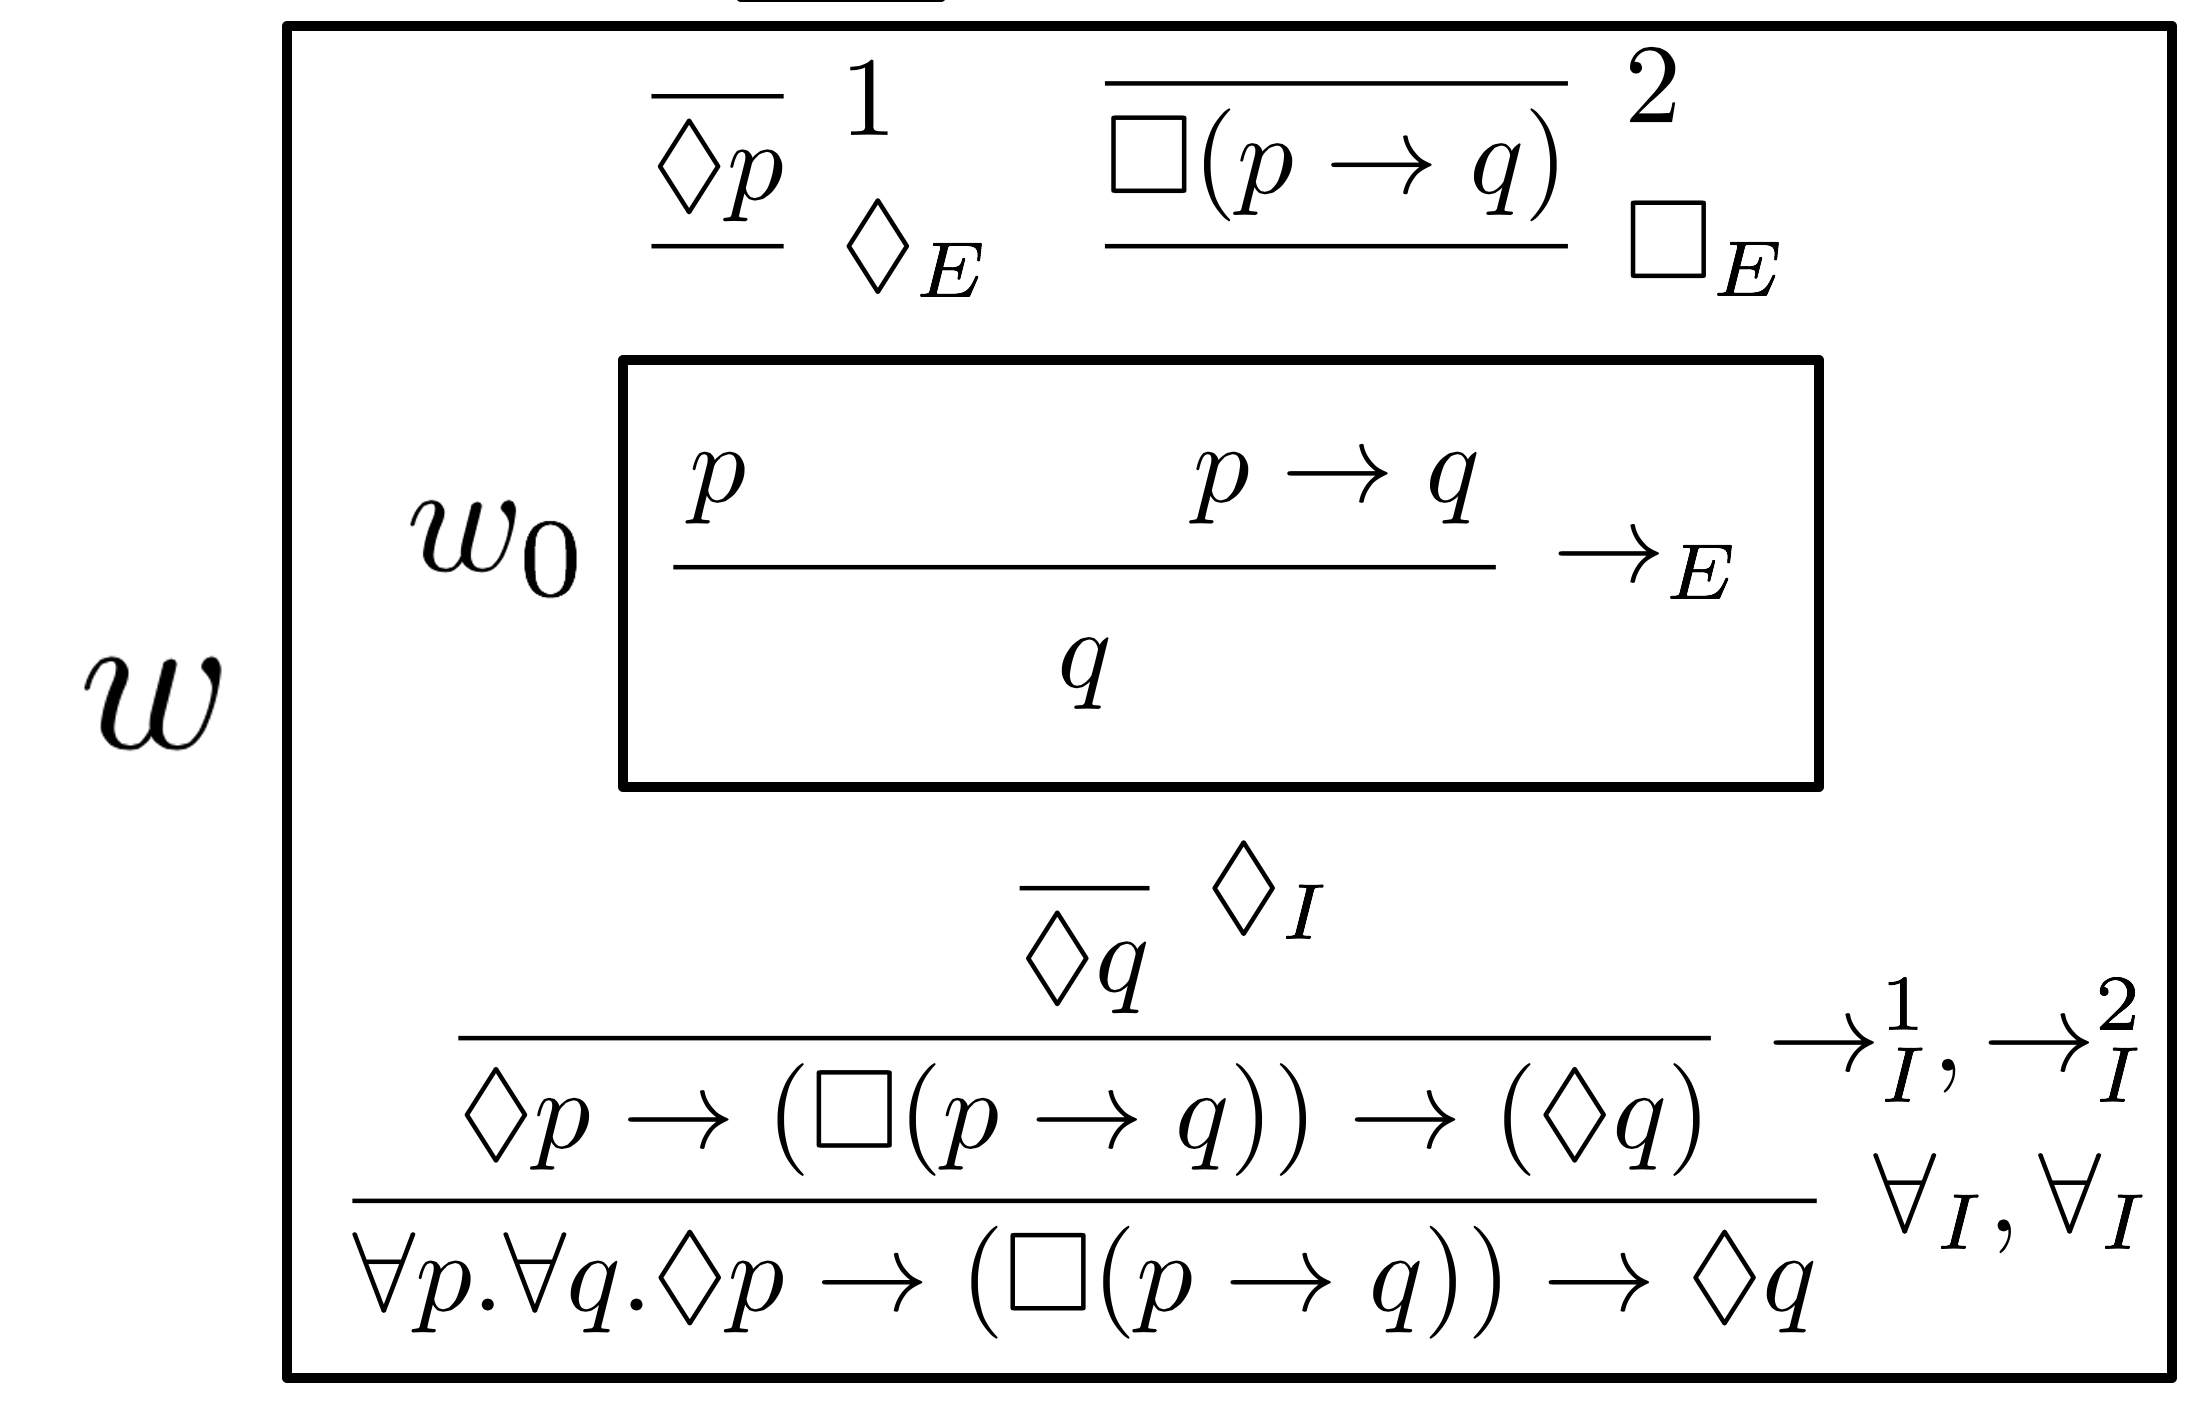
\includegraphics[width=0.5\textwidth]{ND-(mp_dia).png}
\caption{ND proof of \texttt{mp\_dia}\label{fig:mp_dia}}
\end{figure}

\noindent
The same lemma could be proved without the new modal tactics, as shown below.
But this is clearly disadvantageous, for several reasons: 
the proof script becomes longer;
the definitions of modal operators must be unfolded, 
either explicitly (as done below) or implicitly in the user's mind; 
tactic applications dealing with modal operators cannot be easily distinguished
from tactic applications dealing with quantifiers; and  
hypotheses about the reachability of worlds (e.g. \texttt{R1} below) 
must be handled explicitly. In summary, without the modal tactics, 
a convenient and intuitive correspondence between proof scripts and 
modal ND proofs would be missing.

\begin{Verbatim}[commandchars=\\\{\},fontsize=\verbsize]
\Lemma mp_dia_alternative: 
  [mforall p, mforall q, (dia p) m-> (box (p m-> q)) m-> (dia q)].
\Proof. mv. 
intros p q H1 H2. unfold dia. unfold dia in H1. unfold box in H2.
destruct H1 as [w0 [R1 H1]]. exists w0. split.
  exact R1.
  apply H2.
    exact R1.
    exact H1.
\Qed.
\end{Verbatim}


\noindent
The second useful lemma allows negations to be pushed inside modalities, 
and again the modal tactics allow this to be proved conveniently and elegantly.

\begin{Verbatim}[commandchars=\\\{\},fontsize=\verbsize]
\Lemma not_dia_box_not: [mforall p, (m~ (dia p)) m-> (box (m~ p))].
\Proof. mv. 
intro p. intro H. box_i. intro H2. apply H. dia_i w0. exact H2. 
\Qed.
\end{Verbatim}


\section{Modal Logics beyond K}
\label{sec:BeyondK}

The embedding described in Section \ref{sec:Embedding} and the 
new tactics described in Section \ref{sec:Tactics} allow convenient 
interactive reasoning for modal logic \textbf{K} within \Coq. 
The axiom K is easily derivable:

\begin{Verbatim}[commandchars=\\\{\},fontsize=\verbsize]
\Theorem K: 
  [ mforall p, mforall q, (box (p m-> q)) m-> (box p) m-> (box q) ].
\Proof. mv. 
intros p q H1 H2. box_i. box_e H1 H3. apply H3. box_e H2 H4. exact H4. 
\Qed.
\end{Verbatim}

\noindent
For other modal logics beyond \textbf{K}, their frame conditions, which constrain 
the reachability relation, must be stated as \Coq axioms.

\begin{Verbatim}[commandchars=\\\{\},fontsize=\verbsize]
\Axiom reflexivity: \fforall w, r w w.

\Axiom transitivity: \fforall w1 w2 w3, (r w1 w2) -> (r w2 w3) -> (r w1 w3).

\Axiom symmetry: \fforall w1 w2, (r w1 w2) -> (r w2 w1).
\end{Verbatim}

\noindent
Hilbert-style modal logic axioms, such as for example T, 
can be easily derived from their corresponding frame conditions:

\begin{Verbatim}[commandchars=\\\{\},fontsize=\verbsize]
\Theorem T: [ mforall p, (box p) m-> p ].
\Proof. mv. 
intro p. intro H. box_e H H1. exact H1. apply reflexivity. 
\Qed.
\end{Verbatim}

\noindent
In a strong modal logic such as \textbf{S5} (which requires all three frame conditions specified above), sequences of modal operators can be collapsed to a single modal operator. One such collapsing principle is specified and proven below. By applying it iteratively, any sequence $\pos \ldots \pos \nec p$ could be collapsed to $\nec p$.

\begin{Verbatim}[commandchars=\\\{\},fontsize=\verbsize]
\Theorem dia_box_to_box: [ mforall p, (dia (box p)) m-> (box p) ].
\Proof. mv. 
intros p H1. dia_e H1. box_i. box_e H1 H2. exact H2. eapply transitivity. 
  apply symmetry. exact R. 
  exact R0.
\Qed.
\end{Verbatim}


\section{G\"odel's Ontological Argument for God's Existence}
\label{sec:proof}

In order to demonstrate the efficacy and convenience of the modal
embedding approach not only for proving simple lemmas and theorems,
but also for larger developments, we include here a full and detailed
formalization of G\"odel's ontological argument.

Attempts to prove the existence (or non-existence) of God by means of
abstract ontological arguments are an old tradition in philosophy and
theology. G\"{o}del's proof 
%\cite{Goedel1970,GoedelNotes} 
\cite{Goedel1970} 
is a modern
culmination of this tradition, following particularly the footsteps of
Leibniz. Various slightly different versions of axioms and definitions
have been considered by G\"{o}del and by several philosophers who
commented on his proof (cf.
%\cite{sobel2004logic,AndersonGettings,Fitting,Adams,ContemporaryBibliography}).
\cite{sobel2004logic,Fitting,ContemporaryBibliography}).
The formalization shown in this Section aims at being as similar as
possible to Dana Scott's version of the proof \cite{ScottNotes}. The
formulation and numbering of axioms, definitions and theorems is the
same as in Scott's notes. Even the \Coq proof scripts follow precisely
all the steps in Scott's notes. Scott's assertions are emphasized
below with comments. In contrast to the formalization in \Isabelle
\cite{AFP}, where automation via \texttt{Metis}
%\cite{Hurd03first-orderproof} 
and \texttt{Sledgehammer}
%\cite{Sledgehammer} 
using tools such \texttt{LEO-II} \cite{LEO-II} and \texttt{Satallax}
\cite{Satallax} has been successfully employed, the formalization in
\Coq used no automation. This was a deliberate choice, mainly because
it allowed a qualitative evaluation of the convenience of the
embedding approach for \emph{interactive} theorem proving. Moreover,
in order to formalize exactly Scott's version and not some arbitrary
version found automatically\footnote{The proofs found automatically
  by the above provers indeed differ from the one presented here:
  e.g., the strong S5 principle used below (and by Scott) is not needed; the
  ATP proofs only rely on axiom B.}, automation would have to be
heavily limited anyway. Furthermore, the deliberate preference for
simple tactics (mostly \emph{intro}, \emph{apply} and the modal
tactics described in Section \ref{sec:Tactics}) results in proof
scripts that closely correspond to common ND
proofs. This hopefully makes the formalization more accessible to
those who are not experts in \Coq's tactics but are nevertheless
interested in G\"odel's proof.

G\"odel's proof requires \Coq's classical logic libraries as well as the
\texttt{Modal} library developed by us and described in Sections
\ref{sec:Embedding} and \ref{sec:Tactics}.

\begin{Verbatim}[commandchars=\\\{\},fontsize=\verbsize]
\Require \Import Coq.Logic.Classical Coq.Logic.Classical_Pred_Type Modal.
\end{Verbatim}

\noindent 
In Scott's notes, classicality occurs in uses of the
principle of proof by contradiction. In order to clearly
indicate where classical logic is needed in the proof scripts, a
simple tactic that simulates proof by contradiction was created:

\begin{Verbatim}[commandchars=\\\{\},fontsize=\verbsize]
\Ltac proof_by_contradiction H := apply NNPP; intro H.
\end{Verbatim}


\noindent
G\"odel's theory has a single higher-order constant, \texttt{Positive}, 
which ought to hold for properties considered \emph{positive} in a moral sense.

\begin{Verbatim}[commandchars=\\\{\},fontsize=\verbsize]
\com{(* Constant predicate that distinguishes positive properties *)}
\Parameter Positive: (u -> o) -> o.
\end{Verbatim}

\noindent
God is defined as a being possessing all positive properties, and
five axioms are stated to characterize positivity. 
The first part of the proof culminates in \texttt{corollary1} and establishes
that God's existence is possible.


\begin{Verbatim}[commandchars=\\\{\},fontsize=\verbsize]
\com{(* Axiom A1 (divided into two directions):} 
\com{   either a property or its negation is positive, but not both *)}
\Axiom axiom1a : 
  [ mforall p, (Positive (\fun x: u => m~(p x))) m-> (m~ (Positive p)) ].

\Axiom axiom1b : 
  [ mforall p, (m~ (Positive p)) m-> (Positive (\fun x: u => m~ (p x))) ].

\com{(* Axiom A2: }
\com{   a property necessarily implied by a positive property is positive *)}
\Axiom axiom2: [ mforall p, mforall q, 
  Positive p m/\bslash (box (mforall x, (p x) m-> (q x) )) m-> Positive q ].

\com{(* Theorem T1: positive properties are possibly exemplified *)}
\Theorem theorem1: [ mforall p, (Positive p) m-> dia (mexists x, p x) ].
\Proof. mv.
intro p. intro H1. proof_by_contradiction H2. apply not_dia_box_not in H2.
assert (H3: ((box (mforall x, m~ (p x))) w)). \com{(* Scott *)}
  box_i. intro x. assert (H4: ((m~ (mexists x : u, p x)) w0)).
    box_e H2 G2. exact G2.
    clear H2 R H1 w. intro H5. apply H4. exists x. exact H5.
  assert (H6: ((box (mforall x, (p x) m-> m~ (x m= x))) w)). \com{(* Scott *)}   
    box_i. intro x. intros H7 H8. box_elim H3 w0 G3. eapply G3. exact H7.
    assert (H9: ((Positive (fun x => m~ (x m= x))) w)). \com{(* Scott *)}
      apply (axiom2 w p (fun x => m~ (x m= x))). split.
        exact H1.
        exact H6.
      assert (H10: ((box (mforall x, (p x) m-> (x m= x))) w)). \com{(* Scott *)}
        box_i. intros x H11. reflexivity.
        assert (H11 : ((Positive (fun x => (x m= x))) w)). \com{(* Scott *)}
          apply (axiom2 w p (fun x => x m= x )). split.
            exact H1.
            exact H10.
          apply axiom1a in H9. contradiction.
\Qed.

\com{(* Definition D1: }
\com{   God: a God-like being possesses all positive properties *)}
\Definition G(x: u) := mforall p, (Positive p) m-> (p x).

\com{(* Axiom A3: the property of being God-like is positive *)}
\Axiom axiom3: [ Positive G ].

\com{(* Corollary C1: possibly, God exists *)}
\Theorem corollary1: [ dia (mexists x, G x) ]. 
\Proof. mv. apply theorem1. apply axiom3. \Qed.
\end{Verbatim}

\noindent 
The second part of the proof consists in showing that if
God's existence is possible then it must be necessary
(\texttt{lemma2}). The controversial \textbf{S5} principle
\texttt{dia\_box\_to\_box} is used.

\begin{Verbatim}[commandchars=\\\{\},fontsize=\verbsize]
\com{(* Axiom A4: positive properties are necessarily positive *)}
\Axiom axiom4: [ mforall p, (Positive p) m-> box (Positive p) ].

\com{(* Definition D2: }
\com{   essence: an essence of an individual is a property possessed by it} 
\com{   and necessarily implying any of its properties *)}
\Definition Essence(p: u -> o)(x: u) := 
    (p x) m/\bslash mforall q, ((q x) m-> box (mforall y, (p y) m-> (q y))).
\Notation "p 'ess' x" := (Essence p x) (at level 69).

\com{(* Theorem T2: being God-like is an essence of any God-like being *)}
\Theorem theorem2: [ mforall x, (G x) m-> (G ess x) ].
\Proof. mv. intro g. intro H1. unfold Essence. split.
  exact H1.
  intro q. intro H2. assert (H3: ((Positive q) w)).
    proof_by_contradiction H4. unfold G in H1. apply axiom1b in H4. 
    apply H1 in H4. contradiction. 
    
    cut (box (Positive q) w). \com{(* Scott *)}
      apply K. box_i. intro H5. intro y. intro H6. 
      unfold G in H6. apply (H6 q). exact H5.

      apply axiom4. exact H3.
\Qed.

\com{(* Definition D3: }
\com{   necessary existence: necessary existence of an individual }
\com{   is the necessary exemplification of all its essences *)}
\Definition NE(x: u) := mforall p, (p ess x) m-> box (mexists y, (p y)).

\com{(* Axiom A5: necessary existence is a positive property *)}
\Axiom axiom5: [ Positive NE ].

\Lemma lemma1: [ (mexists z, (G z)) m-> box (mexists x, (G x)) ].
\Proof. mv. 
intro H1. destruct H1 as [g H2]. cut ((G ess g) w). \com{(* Scott *)}
  assert (H3: (NE g w)).       \com{(* Scott *)}
    unfold G in H2. apply (H2 NE). apply axiom5.
    unfold NE in H3. apply H3.
  apply theorem2. exact H2.
\Qed.

\Lemma lemma2: [ dia (mexists z, (G z)) m-> box (mexists x, (G x)) ].
\Proof. mv. 
intro H. cut (dia (box (mexists x, G x)) w).  \com{(* Scott *)}
  apply dia_box_to_box.
  apply (mp_dia w (mexists z, G z)).
    exact H.
    box_i. apply lemma1.
\Qed.

\com{(* Theorem T3: necessarily, a God exists *)}
\Theorem theorem3: [ box (mexists x, (G x)) ].
\Proof. mv. apply lemma2. apply corollary1. \Qed.

\com{(* Corollary C2: There exists a god *)}
\Theorem corollary2: [ mexists x, (G x) ].
\Proof. mv. apply T. apply theorem3. \Qed.
\end{Verbatim}


\section{Conclusions}
\label{sec:conclusions}

The successful formalization of Scott's version of  G\"odel's
ontological argument indicates that the \emph{embedding} of
higher-order modal
logics into higher-order logics via the \emph{possible world
semantics} is a viable approach for fully interactive theorem proving
within modal logics. Our lightweight implementation of the embedding
(available in \cite{FormalTheologyRepository} and described 
in Sections \ref{sec:Embedding} and \ref{sec:Tactics})
takes special care to hide the underlying possible world machinery
from the user. An inspection of the proof scripts in Section
\ref{sec:proof} shows that this goal has been achieved. The user does
not have to explicitly bother about worlds and their mutual
reachability; the provided tactics for modalities do the job for
him/her. Moreover, for subgoals that do not involve modalities, the
user has all the usual interactive tactics at his/her disposal.

Although fully automated (as opposed to interactive) theorem proving
is beyond the scope of this paper, it is worth mentioning that all
lemmas and theorems in Sections \ref{sec:Embedding},
\ref{sec:SimpleExamples} and \ref{sec:BeyondK} (but not \ref{sec:proof}) could have been proven
automatically using \Coq's \texttt{firstorder} tactic. The
implementation of hints to allow \Coq's automatic tactics to take full
advantage of the embedding and the modal axioms still remains for
future work. 

The theological implications of the verified correctness of G\"odel's
proof certainly depend on a critical discussion of the underlying
concepts, definitions and axioms, which is beyond the scope of this
paper.  Clearly, the application of theorem proving technology to the
domain of theoretical philosophy can --- as already pictured by
Leibniz --- be very fruitful for both areas. 

The infrastructure that we have implemented for interactive and
automated reasoning in higher-order modal logics is clearly
useful also outside philosophy; the range of potential applications is very wide. 


\paragraph{Acknowledgements:} We thank Cedric Auger and Laurent Th\'ery, 
for their answers to our questions about Ltac in the Coq-Club mailing-list. 


\footnotesize
\bibliographystyle{plain}
\bibliography{Bibliography}


\end{document}